\documentclass{amsart}
\usepackage{tikz, mathpazo, graphicx}
\linespread{1.2}

\title{Problem Set 1 Solutions \\ MAS341: Graph Theory }

\begin{document}
\maketitle
\section{Question 1}
Find a Hamiltonian cycle in the following graph:

\begin{center}
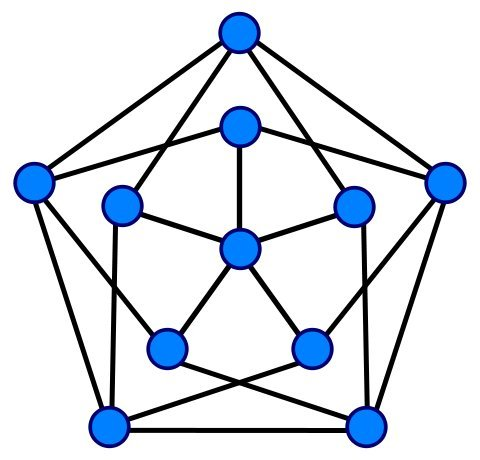
\includegraphics[width=8cm]{ProblemSet1Graph1.jpg}
\end{center}


\begin{proof}
Can be done by trial an error.  Here we find the path using some helpful observations.

 Up to symmetry, there are two possibilities for the path as it goes through the central vertex: either it comes and leaves by two vertices next to each other on the circle (for example, the green edges in the next graph) , or it by vertices not next to each other on the circle (for example, the red edges in the next graph).  

\begin{center} 
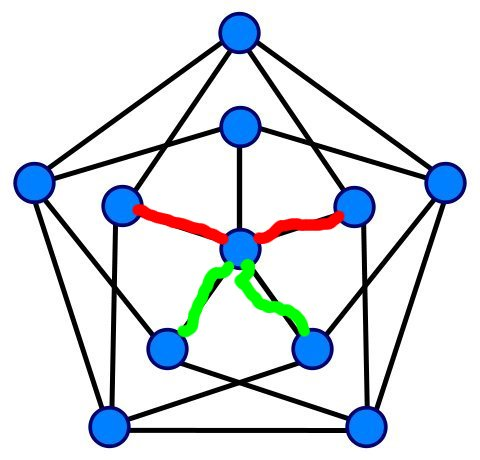
\includegraphics[width=8cm]{PS1RG.jpg}
\end{center}


In any case, the path will visit two of the 5 vertices adjacent to the central vertex, and miss 3 of these vertices.  Since these vertices all have degree 3 -- for the three vertices adjacent to the central vertex in the graph, but not in the Hamiltonian cycle, we then know that any Hamiltonian path must use the other two edges in this ring.  If we consider the case where the path at the central vertex does not use edges ``next'' to each other, we get see that the path must use all the red edges in the following graph:

\begin{center} 
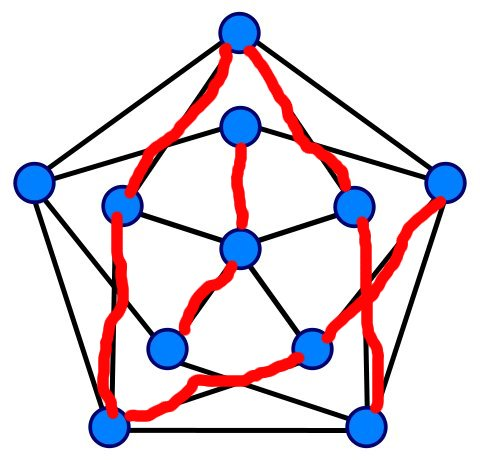
\includegraphics[width=8cm]{PS1S1.jpg}
\end{center}

Now consider how the Hamiltonian path behaves at the leftmost vertex.  It cannot use the edges in the outer pentagon, as those both go to edges that the Hamiltonian path already enters and leave.  Hence it must use teh two edges going into the middle layer, but this makes a cycle of length 4, not using all the vertices.  

Hence, the Hamiltonian path must leave and enter the central vertex from consecutive edges.  As in the previous case, we then now the behavior of the Hamiltonian cycle at the other 3 vertices in the middle ring, and from there onyl a few possibilities are left to investigate, leading to a solution similar to teh following:


\begin{center} 
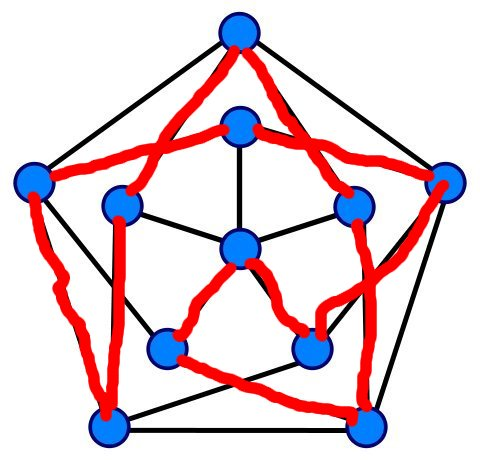
\includegraphics[width=8cm]{PS1P1Sol.jpg}
\end{center}



\end{proof}

\section{Question 2}
Prove that the following graph is not Hamiltonian:


\begin{center} 
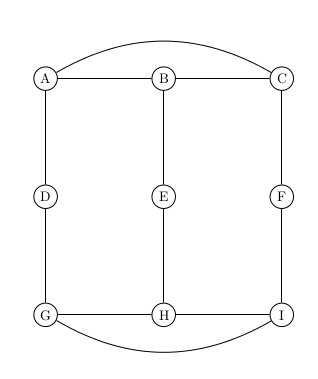
\includegraphics[width=8cm]{ProblemSet1Graph2.jpg}
\end{center}

\subsection{Proof 1:}

Since the vertices $D, E$ and $F$ all have degree two, we know the Hamiltonian path must pass straight through each of them, yielding the following:

\begin{center} 
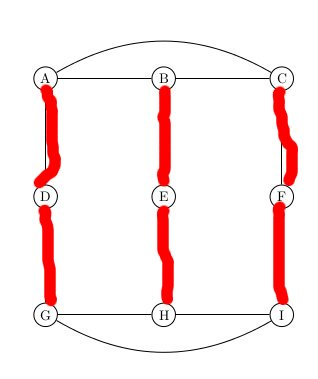
\includegraphics[width=8cm]{PS1S2.jpg}
\end{center}

Now consider how the path continues at vertex $A$ -- either it can go to vertex $B$ or vertex $C$.  If it goes to vertex $B$, then there is nowhere else for the path to go to from vertex $C$, and similarly, if $A$ is connected to $C$, there is nowhere else for the path to connect to at vertex $B$.

\subsection{Proof 2:}

Since the middle vertices $D$, $E$, $F$ all have degree two, the path throw these must connect the ``top'' ($A, B, C$) to the ``bottom'' ($G, H I$).

Consider the path starting from $A$ -- it must pass throw each of $D, E, F$ exactly once, and hence must switch between the top and bottom of the graph exactly three times.  This means it would end on the bottom, and be unable to connect back to vertex $A$.

\subsection{Proof 3:}
This proof starts by mimicing the proof that the Petersen graph is not Hamiltonian.

The graph has 9 vertices and 12 edges, so if there were a Hamiltonian cycle, it would use all but three edges.  The Hamiltonian cycle would be a 9-cycle; each of these additional edges would ``split'' the nine cycle into two cycles, with total length 11 (since the two vertices on the ``new'' edges are each used twice).  Since the graph is simple, there are no loops or multiple edges, and hence the possibilities are a 3 cycle and an 8 cycle, a 4 cycle or a 7 cycle, or a 5-cycle and a 6-cycle.  See the pictures in Lecture 

The graph has no 4 or 5 cycles, and hence each edge must split it into a 3 cycle and an 8 cycle.  However, we need to add 3 edges, each making a 3 cycle, but the graph itself only has 2 three cycles, and hence the graph cannot have a Hamiltonian cycle. 

Other arguments at the end can also work.


\section{Question 3}

We saw in class that $\Gamma$ has a vertex such that removing it disconnects the graph, then $\Gamma$ is not Hamiltonian.  Prove the following generalization:

Suppose that graph $\Gamma$ has $n$ vertices $v_1,\dots, v_n$ so that if we remove all $n$ vertices, the resulting graph $\Gamma\setminus \{v_1,\dots, v_n\}$ has more than $n$ components.  Prove that $\Gamma$ is not Hamiltonian.  



\subsection{Proof 1:}
We prove the contrapositive; and show that if $\Gamma$ is Hamiltonian, 
  Suppose that $\Gamma$ was Hamiltonian; and consider the Hamiltonian cycle as a circle.  When we remove $n$ vertices, we are essentially cutting the circle in $n$ points -- this will make at most $n-1$ pieces (the first cut will not disconnect the graph; every cut after can add at most one component).

\subsection{Proof 2: (Another way or writing essentially the same argument)}

Suppose that $\Gamma\setminus \{ v_1,\dots, v_n\}$ had connected components $C_1,\dots, C_k$, where $k>n$.  If $\Gamma$ had a Hamiltonian path, it would have to pass through each $C_i$ at least once.  Every time it leaves a $C_i$, it has to pass through one of the vertices $\{v_1,\dots, v_n\}$.  Since we have to return to the $C_i$ we start with, we must leave every component at least once, and hence we must use up at least $k$ of the $v_i$, which is a contradiction since $k>n$.




\end{document}
